\chapter{INTRODUCTION TO STATISTICS}
\section*{INTRODUCTION}
This module present a discussion on statistics to include key concepts, uses and
importance of statistics and probability, data collection and the different forms of data
representation. It will also discuss the measures of central tendency for ungrouped and grouped
data. Every lesson will present examples, application and sample assessment tools. You will
appreciate more the importance of statistics which you will also share to your students.
\section*{OBJECTIVES}
After completing this module, you should be able to:
\begin{enumerate}
\item Explain the basic concepts, uses, and the branches of statistics;
\item Collect or gather statistical data and organize in a frequency table according to some
systematic considerations;
\item Use appropriate graph to represent organized data: pie, bar graph, line graph, and
histogram;
\item Analyze, interpret accurately and draw conclusions from graphic and tabular
presentations of statistical data;
\item Find the mean, median and mode of statistical data; and
\item Describe the data using information from the mean, median and mode.
\end{enumerate}
\section*{DISCUSSION}
\begin{definition}[Statistics]
\Bold{Statistics} is the science of conducting studies to collect, organize, summarize,
analyze and draw conclusions from data (Bluman, 2004). It is a science of
collection and classification of facts in the basis of relative number or
occurrence.
\end{definition}
The \Bold{collection} or \Bold{gathering of data} may be undertaken using interview, questionnaires,
tests, observation, registration, and experiments. \Bold{Organization of data} is the manner of
presenting the gathered data into tabular, textual or graphical form. The \Bold{summarized data} will
be subjected to \Bold{analysis} in order to extract relevant data and information using statistical tools
or techniques. \Bold{Interpretation of data} refers to the drawing of conclusions or inferences from
the analyzed data (Basilio, Faith B., Edna A. Chua, Maria T. Juwanan, 2003).
\subsection*{Uses of Statistics}
Statistics has many uses. Among the contributions of statistics are the following:
\begin{itemize}
\item Statistics provides us with the ways and means of expressing our thoughts in the most
definite and exact way feasible. Example: There are more females in the first year than
males; it will rain on June.
\item Statistics provides us with numbers and figures with which to describe completely and
   accurately the characteristics of certain phenomena. Example: There are 25 females in
  the first year and 20 are males; it will rain on June 10.
\item Statistics enables us to express the results of research activities meaningfully and
   present them in a form easily understood and read. Example: in tables or graphs.
\item Statistics allows us to draw inferences or conclusions from characteristics of given data.
\end{itemize}

In \textcite{psasrtc}, it was mentioned
that the eminent statistician Bradley Efron summarized how diverse the uses of
statistics: % Consider revising. Sounds pedantic.
\begin{Quote}
During the 20th Century statistical thinking and methodology has
become the scientific framework for literally dozens of field including
education, agriculture, economics, biology, and medicine, and with
increasing influence recently on the hard sciences such as astronomy,
geology, and physics. In other words, we have grown from a small
obscure field into a big obscure field.
\end{Quote}
\subsection*{BRANCHES OF STATISTICS}
There are two areas of statistics namely: descriptive statistics and inferential
statistics.
\begin{definition}[Descriptive Statistics]
\Bold{Descriptive Statistics} tend to bring out into light only the significant aspects of data.
A large mass of data come into man's hands for his use. Oftentimes these data are
complex that yield so much information.
\end{definition}
\begin{example}
\Item the rating obtained by the senior students of public high schools in the
National College Entrance Examination will yield an almost unlimited amount of information
such as: the highest ratings; the lowest rating; the most frequent rating; the range of the ratings;
the number of students who belong to the upper 75\%, 50\%, or 25\% of the group; and many
more.
%Consider making this part more concise
\end{example}
\begin{definition}[Inferential Statistics]
\Bold{Inferential Statistics} is concerned in drawing conclusions or inferences or from the
given characteristics of the samples to specific properties of the population. In
inferential statistics, testing the significant difference and independence between
two or more variables are given emphasis. An assertion or hypothesis about the
population is made and is intended to be rejected or accepted depending on the
result of a test based from available samples. % Consider fixing grammar and usage
\end{definition}
Before we proceed with the discussion of statistics, there are some terms commonly used in
statistics that we have to define.
\begin{definition}[Universe, Variable, Parameters]
The \Bold{universe} or \Bold{population} is the set of all entities under study. Meanwhile, a \Bold{variable}
is the attribute of interest observable of each entity in the universe. Parameters are
numerical measures that describe the population of interest. Example, you can
consider all the students in 7-Quartz as the population, a possible variable is their
math grade, while a possible parameter is the average math grade of the class \parencite{psasrtc}.
\end{definition}
The \textit{population} refers to groups or aggregates of people, animals, objects, materials,
happenings or things of any form \parencite{punzalan}. While \Bold{sample} is a subset or a
representative group of a population to represent the characteristics or traits \parencite{basilio}. For example, in a baranggay with 5,000 families, a sample could be a group of 100
families.

A \Bold{parameter} is any measure of a given characteristic of the \textit{entire} population, for
example the average number of children in each family in a certain baranggay. On the other
hand, a \Bold{statistic} is any measure of a given characteristics based on a \textit{part (sample)} of a
population under study. Example, the corresponding statistic to the previous example is the
average number of children in a sample of 100 from a population of 5,000 families.

\subsubsection*{VARIABLES AND TYPES OF DATA}
The building blocks of statistical science are data \parencite{psasrtc}.
\begin{definition}[Data]
\Bold{Data} are the values (measurement or observations) that the variables can assume \parencite{bulman}. \Bold{Variables} refer to the fundamental quantity that changes/vary in value from one observation to another within a given domain and under given set of conditions \parencite{delrosario}. Quantities that do not take different values from one observation to another are called constants. Variables can be classified as \Bold{quantitative} and \Bold{qualitative}. Quantitative are numerical data while qualitative are categorical data. % Expound on categorical data.
\end{definition}
Some examples of quantitative variables are age, height, weight, scores in the exam,
and temperature. Examples of qualitative data include food preference, student's section, city
address, favorite color, and favorite subject.
\subsubsection*{PRESENTATION OF DATA}
Data gathered can be presented in many ways: tabular, graphical and
even textual. In this section, it will present the mechanics on how to present
data using frequency distribution, histogram, frequency polygon, bar graph,
line graph, and pie chart.
\begin{definition}[Frequency distribution]
A \Bold{frequency distribution} is the organization of raw data in table form, using
classes and frequencies \parencite{bulman}.
\end{definition}
% The construction of frequency distribution for qualitative data needs an overhaul.
\Bold{Frequency Distributions for qualitative} data look like tallies of the number of data that
corresponds to the different values of the variable.
\begin{example}
\Item A social worker wanted to determine the religious affiliation of twenty
families in a certain barangay. The data set is

\begin{tabularu}{llll}
Aglipayan & Protestant & Roman Catholic & Muslim\\
Born Again Christian & Aglipayan & Protestant & Roman Catholic\\
Aglipayan & Muslim & Protestant & Roman Catholic\\
Roman Catholic & Protestant & Roman Catholic & Roman Catholic\\
Roman Catholic & Protestant & Roman Catholic & Roman Catholic\\
\end{tabularu}

To make a table which summarizes the data, follow these steps:
\begin{enumerate}
\item Make a table as shown.
\end{enumerate}
\begin{tabular}{cccc}
\hline
A & B & C & D \\
Class & Tally & Frequency & Percent\\
\parbox[t]{0.2\linewidth}{\raggedright
Aglipayan\\
Protestant\\
Roman Catholic\\
Born Again\\
Christian\\
Muslim
} & & & \\
\hline
 & Total & (n) &  \\
\end{tabular}
\item Tally the data and place the results in column B.
\item Count the tallies and place the corresponding frequency in column C.
\item Find the percentage in each class by using the formula:
\begin{equation*}
\text{Percentage}=\frac{f}{n}\cdot 100\%
\end{equation*}
\item Find the totals for column C and D to complete the table.
\begin{center}
\captionof{table}{A Distribution of the Religious Affiliation of Twenty Families}
\begin{tabular}{cccc}
\hline
A & B & C & D \\
Class & Tally & Frequency & Percent\\
Aglipayan & \tally{3} & 3 & 15\\
Protestant & \tally{5} & 5 & 25\\
Roman Catholic & \tally{9} & 9 & 45\\
Born Again Christian & \tally{1} & 1 & 5\\
Muslim & \tally{2} & 2 & 10\\
\hline
 & Total ($n$) & 29 & 100 \\
\end{tabular}
\end{center}
So from the given example, more families are affiliated with Roman Catholic than any
other religion.
\end{example}

\Bold{Frequency Distributions for Quantitative Data} are also called Grouped Distributions. This
is because data which are close enough are grouped into one and these groups are called
\Bold{classes}. Each class has a \Bold{lower class limit} and an \Bold{upper class limit} which serve as guides as to which data will be counted to each class. The \Bold{class boundaries} are the midpoints of the
upper class limits of one class and the lower class limit of the next class. The \Bold{class width} is
the difference between two successive class boundaries. It also corresponds to the
difference between two successive lower class limits or two successive upper class limits.
The \Bold{class mark} is the midpoint of each class. The \Bold{cumulative frequency} is a continuous
tally of the frequencies. Here's an example of a Quantitative Frequency Distribution:
\begin{center}
\captionof{table}{Distribution of Math Long Test Scores of a sample of 24 students}
\begin{tabularu}{ccccccc}
\hline \hline
Lower & Upper & Lower Class & Upper Class & Class & Frequency & Cumulative \\
Class Limit & Class Limit & Boundary & Boundary & Mark &  & Frequency\\
\hline
10 & 14 & 9.5 & 14.5 & 12 & 4 & 4\\
15 & 19 & 14.5 & 19.5 & 17 & 9 & 13\\
20 & 24 & 19.5 & 24.5 & 22 & 6 & 19\\
25 & 29 & 24.5 & 29.5 & 27 & 5 & 24\\
\hline
\end{tabularu}
\end{center}
\begin{example}
\Item Given the scores of sophomore students in Mathematics 1 periodical test,
construct the frequency distribution.

\begin{tabularu}{llllllllll}
50 & 55 & 60 & 41 & 34 & 58 & 37 & 35 & 56 & 59\\
48 & 20 & 65 & 63 & 61 & 28 & 36 & 55 & 53 & 60\\
33 & 45 & 56 & 60 & 42 & 56 & 41 & 45 & 57 & 59\\
\end{tabularu}

\Solution

\begin{myenumerate}
\item Find the \Bold{range} by using the formula:
\begin{align*}
\text{Range}&=\text{Highest Score}-\text{Lowest Score}\\
 &=65-20\\
 &=\boxed{45}
\end{align*}
\item Determine the \Bold{number of classes} ($k$). The ideal number of class intervals is between 5
and 20 depending on the nature of data. You can also use the formula to determine
the number of intervals
\begin{align*}
k&=\sqrt{n}\\
k&=\sqrt{30}\\
 &=5.4\\
 &\approx 5
\end{align*}
Another way of finding the number of intervals is using the \Bold{Sturges' Rule}:
$K = 1 + 3.3\log n$; where n is the number of samples.

For the purposes of this module as Introduction to Statistics, the teacher should set
the number of intervals ($k$). Usually, limit the data to $20-50$, using $4-6$ classes.
\item  Determine the \Bold{class width/interval} ($i$) using this formula:
\begin{align*}
\text{Class Width}\,(i)&=\frac{R}{k}\\
&=\frac{45}{5}\\
&=\boxed{9}
\end{align*}
Usually, the computed value for the class width is not a whole number. If this is the
case, \textit{round up to the nearest whole number}.

If the computed value for the class width is a whole number, consider adding 1. Not
doing so might result to at least one of the data points being excluded in the table.

\item  Determine the \Bold{class limits}. The lower limit of the lowest class should be a multiple of
the class width.

Since $i = 9$ and the lowest score is 20 which is not a multiple of the class
width thus, 18 will be the lower limit. Therefore, the lowest class interval
will be $18 - 26$.

\item  Determine the \Bold{class boundaries} by subtracting 0.5 from each lower class limit and
adding 0.5 to each upper limit: $17.5 - 26.5, 26.5 - 35.5$.

\item Determine the \Bold{class mark/midpoint} of every class. It is obtained by getting the sum of
the lower and upper limits of a class divided by two.
\begin{equation*}
\text{Class Mark}=\frac{18+26}{2}=22
\end{equation*}
\item Tally the data.

\item Find the numerical frequencies from the tallies.

\item Find the cumulative frequencies.

\noindent
\begin{center}
\begin{tabular}{@{}c@{\;}c@{\;}c@{}c@{}c@{\;}c@{}}
\hline \hline
Class Limits & Class & Class & Tally & Frequency & Cumulative\\
 & Boundaries & Marks &  &  & Frequency\\
18 - 26 & 17.5 - 26.5 & 22 & \tally{22} & 1  & 1\\
27 - 35 & 26.5 - 35.5 & 31 & \tally{31} & 4  & 5\\
36 - 44 & 35.5 - 44.5 & 40 & \tally{40} & 5  & 10\\
45 - 53 & 44.5 - 54.5 & 49 & \tally{49} & 5  & 15\\
54 - 62 & 54.5 - 62.5 & 58 & \tally{58} & 13 & 28\\
63 - 71 & 62.5 - 71.5 & 67 & \tally{67} & 2  & 30\\
        &             &    & Total $(n)$ & 30 & \\
\hline
\end{tabular}
\captionof{table}{A Distribution of the Mathematics 1 Periodical Test Scores of Thirty Sophomore Students}
\end{center}
\end{myenumerate}
\end{example}
There are also ways to summarize data in the form of graphs or charts. The main
advantage of using charts and graphs is that they give a visual representation of the data. This
makes interpretation of the data easier compared to just seeing data in tables.

Here are some examples of usual graphs and charts you can use in order to summarize
data.

\begin{definition}[Histogram]
A \Bold{histogram} displays data by using adjacent vertical bars of various heights to
represent the frequencies of the classes. The histogram is a graphical
representation of a frequency distribution table.
\end{definition}
\begin{example}
\Item Construct a histogram to represent the frequency distribution below for the
scores of sophomore students in Mathematics 1 Periodical Test.
\begin{center}
\begin{tabularu}{ccc}
\hline \hline
Class limits & Class & Frequency\\
 & Boundaries & \\
18 - 26 & 17.5 - 26.5 & 1\\
27 - 35 & 26.5 - 35.5 & 4\\
36 - 44 & 35.5 - 44.5 & 5\\
45 - 53 & 44.5 - 54.5 & 5\\
54 - 62 & 54.5 - 62.5 & 13\\
63 - 71 & 62.5 - 71.5 & 2\\
\hline
 & & $n=30$\\
\hline
\end{tabularu}
\end{center}

\Solution

\begin{myenumerate}
\item Draw and label the $x$ and $y$ axes.
\item Represent the frequency on the $y$-axis and the class boundaries on the $x$-axis.
\item Using the frequencies as the heights, draw vertical bars for each class.
\begin{center}
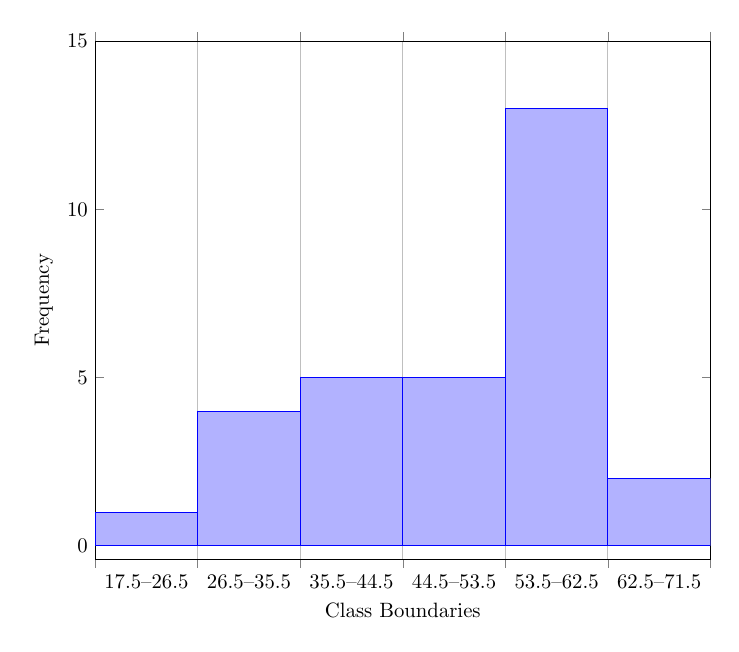
\begin{tikzpicture}[scale=0.75,transform shape]
\begin{axis}[width=12cm,xmin=17.5,xmax=71.5,xlabel=Class Boundaries,ylabel=Frequency,
ybar interval,
xticklabel=
\pgfmathprintnumber\tick--\pgfmathprintnumber\nexttick,
ymax=15,
ytick={0,5,10,15}]
\addplot+[hist={bins=6}]
table[row sep=\\,y index=0] {
data\\
50\\
48\\
33\\
55\\
20\\
45\\
60\\
65\\
56\\
41\\
63\\
60\\
34\\
61\\
42\\
58\\
28\\
56\\
37\\
36\\
41\\
35\\
55\\
45\\
56\\
53\\
57\\
59\\
60\\
59\\
};
\end{axis}
\end{tikzpicture}
\captionof{figure}{Scores of Sophomore Students in Mathematics 1 Periodical Test (Histogram)}
\end{center}
\end{myenumerate}
\end{example}
The histogram presents that the class boundary with the greatest frequency is
54.5 - 62.5 while the lowest is 17.5 - 26.5.
\begin{definition}[Frequency Polygon]
A \Bold{frequency polygon} connects the points representing relevant data in the
coordinate plane.
\end{definition}
\begin{example}
\Item Construct a frequency polygon from the histogram for the scores of
sophomore students in Mathematics 1 Periodical Test.

\Solution

\begin{myenumerate}
\item Draw and label the $x$ and $y$ axes.
\item Represent the frequency on the $y$-axis and the class mark on the $x$-axis.
\item Connect the points.
\begin{center}
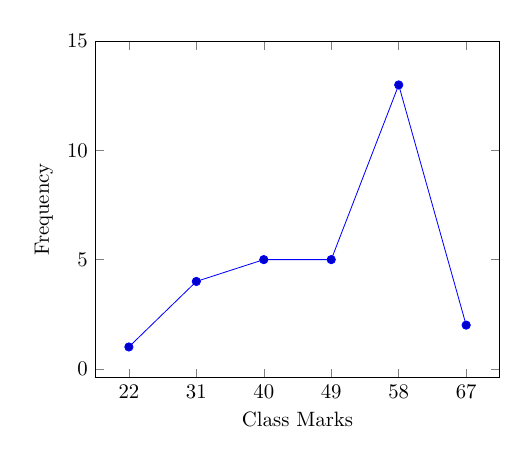
\begin{tikzpicture}[scale=0.75,transform shape]
\begin{axis}[
xtick=data,
mark=,
ymax=15,
xlabel=Class Marks,
ylabel=Frequency,
ytick={0,5,10,15}]
\addplot+[sharp plot] coordinates
{(22,1) (31,4) (40,5) (49,5) (58,13) (67,2)};
\end{axis}
\end{tikzpicture}
\captionof{figure}{Scores of Sophomore Students in Mathematics 1 Periodical Test (Line Graph)}
\end{center}
\end{myenumerate}
\end{example}
\begin{definition}[Bar Graph]
A \Bold{bar graph} is an illustration of the data using bars in the coordinate plane.
This can be used for quantitative data. % Verify that bar graphs are only used for qualitative data.
\end{definition}
\begin{example}
\Item The table shows the educational attainment distribution of parent-respondents.
\begin{center}
\begin{tabularu}{ll}
\hline \hline
Educational Attainment & Frequency\\
\hline
High School Graduate & 10\\
College Graduate & 23\\
MA/MS Graduate & 5\\
PhD Graduate & 3\\
\hline
\end{tabularu}
\end{center}
\Solution

\begin{myenumerate}
\item Draw and label the $x$ and $y$ axes.
\item Represent the frequency on the $y$-axis and the category on the $x$-axis.
\item Draw the bars for each class. Place corresponding category on top of the bars.
\begin{center}
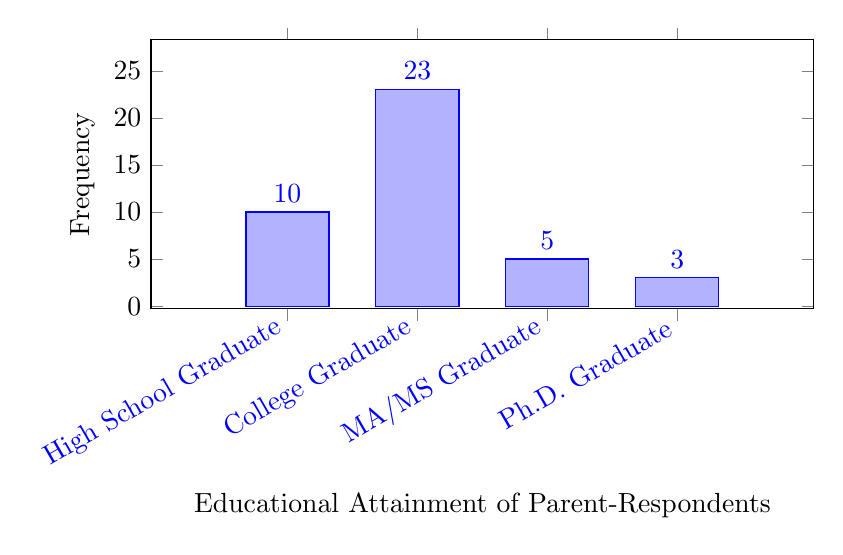
\begin{tikzpicture}
\begin{axis}[
ybar,
width=10cm, 
height=5cm, 
enlarge y limits=0.15, enlarge x limits=0.35,
xlabel={Educational Attainment of Parent-Respondents},
ylabel={Frequency},
symbolic x coords={High School Graduate, College Graduate, MA/MS Graduate, Ph.D. Graduate},
xtick=data,
nodes near coords, nodes near coords align={vertical},
x tick label style={rotate=30,anchor=east,color=blue},
ymax=25,
ytick={0,5,10,15,20,25},
bar width=30pt,
]
\addplot coordinates {(High School Graduate,10) (College Graduate,23) (MA/MS Graduate,5) (Ph.D. Graduate,3)};
\end{axis}
\end{tikzpicture}
\end{center}
\end{myenumerate}
The bar graph shows that \textit{College Graduate} had the highest frequency and Ph D graduate
the lowest.
\end{example}
\begin{definition}[Pie Chart]
A \Bold{pie chart} is a circle that is divided into sections according to the
percentage of frequencies in each category of the distribution. This is
usually used to show the different components of the population.
\end{definition}
\begin{example}
\Item The table below shows the enrolment data of PSHS-Ilocos Region
Campus for School Year 2011 – 2012. Construct a pie graph for the data.
\begin{center}
\begin{tabular}{ll}
\hline \hline
Year Level Frequency\\
\hline
1st Year & 88\\
2nd Year & 78\\
3rd Year & 65\\
4th Year & 48\\
\hline 
\end{tabular}
\end{center}
\Solution
\begin{myenumerate}
\item A circle has $360\degree$, the frequency for each class should be converted into a
proportional part of the circle. The formula is as follows:
\begin{equation*}
\text{Degrees}=\frac{f}{n}\cdot360
\end{equation*}
where $f =$ frequency of each class and $n =$ sum of the frequencies.
\begin{center}
\begin{tabular}{ccc}
\hline \hline 
Year Level & Frequency & Proportional Part\\
\hline 
1st Year & 88 & $\frac{88}{279}\cdot360\degree=113.55\degree\approx 113\degree$\\
2nd Year & 78 & $\frac{78}{279}\cdot360\degree=100.65\degree\approx 101\degree$\\
3rd Year & 65 & $\frac{65}{279}\cdot360\degree=83.87\degree\approx 84\degree$\\
4th Year & 48 & $\frac{48}{279}\cdot360\degree=61.94\degree\approx 62\degree$\\
\end{tabular}
\end{center}
\item Convert the frequency of each class to percentage using the formula:
\begin{equation*}
\%=\frac{f}{n}\cdot100\%
\end{equation*}
\item Draw the graph using a protractor and a compass. Label each section with the name and percentages.
\begin{center}
\begin{tikzpicture}
\pie[radius=1.5,color={blue!80, blue!60, blue!40, blue!20}]{32/1st Year, 28/2nd Year, 23/3rd Year, 17/4th Year}
\end{tikzpicture}
\captionof{figure}{Enrolment Data of PSHS-Ilocos Region Campus for School Year 2011--2012}\label{chap10fig:1}
\end{center}
\end{myenumerate}

From Figure \eqref{chap10fig:1}, it could be observed that the enrolment of freshmen has the
greatest, with 32\% compared to the other year levels.

\item Below is a pie chart showing the population of the four
provinces of Region 1 on 2010. What can you infer? Make necessary
conclusion for this chart.

\begin{center}
\begin{tikzpicture}
\pie[radius=1.5,color={blue!80, blue!60, blue!40, blue!20}]{12/Ilocos Norte, 58/Pangasinan, 16/La Union, 14/Ilocos Sur}
\end{tikzpicture}
\captionof{figure}{Population for Region 1 Based on 2010 Censuses}\label{chap10fig:2}
\end{center}

\Solution

Possible Answers: From the four provinces, Pangasinan has the most number of living
individuals. More than fifty percent of the region's population hales in Pangasinan.
\end{example}
\subsection*{MEASURES OF CENTRAL TENDENCY}
A data can be summarized by using a single number, which is the
concentration point of scores. The three (3) measures of central tendency are the
\Bold{mean}, \Bold{median}, and the \Bold{mode}.

The table below presents the properties of the different measures of central tendency
which was adopted from Bluman \textcite{bulman}.

\begin{center}
\begin{longtable}{>{\bfseries\arraybackslash}cccc}
\hline \hline
Measure & Symbol & Definition & Properties and Uses\\
\hline
\endfirsthead 
\caption[]{(continued)}\\
\hline \hline 
Measure & Symbol & Definition & Properties and Uses\\
\hline
\endhead
\hline 
\multicolumn{4}{r}{Continued to next page\ldots}
\endfoot
\hline
\endlastfoot
Mean & $\mu,\bar{X}$ & \parbox[t]{1in}{\centering
Sum of values,
divided by total
number of
values} & \parbox[t]{0.5\linewidth}{\raggedright
\begin{enumerate}
\item One computes the mean by using all values of the data.
\item The mean varies less than the median or mode when samples
are taken from the same population and all three measures are
computed for these samples.
\item The mean is used in computing other statistics, such as the
variance.
\item The mean for the data set is unique and not necessarily one of
the data values.
\item The mean cannot be computed for an open-ended frequency
distribution.
\item The mean is affected by extremely high or low values, called
outliers, and may not be the appropriate average to use in these
situations.
\end{enumerate}
}\\
Median & MD & \parbox[t]{1in}{
Middle point in
data set that has
been ordered
} & \parbox[t]{0.5\linewidth}{
\begin{enumerate}
\item The median is used when one must find the center or middle
value of a data set.
\item The median is used when one must determine whether the data
values fall into the upper half or lower half of the distribution.
\item The median is affected less than the mean by extremely high or
extremely low values.
\end{enumerate}
}\\
Mode & Mo & \parbox[b]{1in}{Most frequent
data value} & \parbox[t]{0.5\linewidth}{
\begin{enumerate}
\item The mode is used when the most typical case is desired.
\item The mode is the easiest average to compute.
\item The mode can be used when the data are nominal, such as
religious preference, gender, or political affiliation.
\item The mode is not always unique. A data set can have more than
one mode, or the mode may not exist for a data set.
\end{enumerate}
}\\
\hline
\end{longtable}
\end{center}
\begin{example}
\Item The data represent the lengths of service (in years) for a sample of nine (9) PSHS-
IRC teachers. Find the mean, median and mode.
\begin{center}
9,9,8,2,3,5,4,2,7
\end{center}
\Solution

\begin{myenumerate}
\item \Bold{Finding the mean of a list of data}
\begin{align*}
\bar{X}&=\frac{\sum X}{n}\\
 &=\frac{9+9+8+2+3+5+4+2+7}{9}\\
 &=\frac{49}{9}\\
 &=\boxed{5.44}
\end{align*}

Hence, the mean of the length of service (in years) of PSHS-IRC teachers is 5.44
years.

\item \Bold{Finding the median of a list of data}
\begin{description}
\item[Step 1.] Arrange the data in an array (increasing/decreasing order).
\begin{center}
9, 9, 8, 7, 5, 4, 3, 2, 2
\end{center}
\item[Step 2.] Select the middle value. That is the median of the data set.
\begin{center}
9, 9, 8, 7, \tikzmark{5}\phantom{5}, 4, 3, 2, 2
\end{center}
\begin{tikzpicture}[remember picture, overlay]
\node [rectangle,inner sep=1pt,draw] at ([yshift=3pt]5) {5};
\node [below] at (5) {Median};
\useasboundingbox{(5)};
\end{tikzpicture}

Hence, the median length of service (in years) of PSHS-IRC teachers is 5.
\end{description}
This method works only if there is an odd number of data in the set. However,
if the number of data is even, there will be two middle values. To get the
median of that data set, get the average of the two middle values.

Suppose the data set is 9, 9, 8, 7, 6, 5, 4, 3, 2, 2. The two middle values are 6 and
5. So the median is the average of these two numbers, which is 5.5.

\item \Bold{Finding the mode of a list of data}
\begin{description}
\item[Step 1.] Arrange the data in an array (increasing/decreasing order).
\begin{center}
9, 9, 8, 7, 5, 4, 3, 2, 2
\end{center}
\item[Step 2.] Select the value that occurs most often in a data set.

Since, 9 and 2 occur 2 times, the modes are 9 and 2. This data set is said
to be \Bold{bimodal}.

If the data has no repeated value, then there is no mode. Also, if for example all
the values occur twice, thrice or whatever number of times, there is also no
mode.
\end{description}
\end{myenumerate}
\end{example}

\section*{ENRICHMENT LESSON}
\begin{example}
\Item Below is a distribution of Mathematics 1 periodical test scores of thirty
sophomore students. Compute the mean, median and mode.
\begin{center}
\begin{tabular}{ccc}
\hline \hline 
Class Limits & Class & Frequency\\
 & Boundaries & $(f)$\\
\hline
18 - 26 & 17.5 - 26.5 & 1\\
27 - 35 & 26.5 - 35.5 & 4\\
36 - 44 & 35.5 - 44.5 & 5\\
45 - 53 & 44.5 - 54.5 & 5\\
54 - 62 & 54.5 - 62.5 & 13\\
63 - 71 & 62.5 - 71.5 & 2\\
\hline
 & & $n=30$\\
\end{tabular}
\end{center}
\Solution

\begin{myenumerate}
\item \Bold{Finding the mean of grouped data}
\begin{description}
\item[Step 1.] Make a table as shown.
\begin{center}
\begin{tabular}{ccccc}
\hline \hline
A & B & C & D & E\\
Class Limits & Class & Class & Frequency & $f\cdot X_m$\\
 & Boundaries & $(f)$ & Marks & \\
 &  &  & $(X_m)$ & \\
\hline
18 - 26 & 17.5 - 26.5 & 1  & & \\
27 - 35 & 26.5 - 35.5 & 4  & & \\ 
36 - 44 & 35.5 - 44.5 & 5  &  & \\
45 - 53 & 44.5 - 54.5 & 5  &  & \\
54 - 62 & 54.5 - 62.5 & 13 &  & \\
63 - 71 & 62.5 - 71.5 & 2  &  & \\
\hline
 & & $n=30$ & & \\
\end{tabular}
\end{center}

\item[Step 2.] Compute the class marks/ midpoints of each class and complete column D.

\begin{center}
\begin{tabular}{ccccc}
\hline \hline
A & B & C & D & E\\
Class Limits & Class & Class & Frequency & $f\cdot X_m$\\
 & Boundaries & $(f)$ & Marks & \\
 &  &  & $(X_m)$ & \\
\hline
18 - 26 & 17.5 - 26.5 & 1  & 22 & \\
27 - 35 & 26.5 - 35.5 & 4  & 31 & \\ 
36 - 44 & 35.5 - 44.5 & 5  & 40 & \\
45 - 53 & 44.5 - 54.5 & 5  & 49 & \\
54 - 62 & 54.5 - 62.5 & 13 & 58 & \\
63 - 71 & 62.5 - 71.5 & 2  & 67 & \\
\hline
 & & $n=30$ & & \\
\end{tabular}
\end{center}

\item[Step 3.] For each class, multiply the frequency by the class mark, and fill-in
column E.

\begin{center}
\begin{tabular}{ccccc}
\hline \hline
A & B & C & D & E\\
Class Limits & Class & Class & Frequency & $f\cdot X_m$\\
 & Boundaries & $(f)$ & Marks & \\
 &  &  & $(X_m)$ & \\
\hline
18 - 26 & 17.5 - 26.5 & 1  & 22 & 124 \\
27 - 35 & 26.5 - 35.5 & 4  & 31 & 200 \\ 
36 - 44 & 35.5 - 44.5 & 5  & 40 & 200 \\
45 - 53 & 44.5 - 54.5 & 5  & 49 & 245 \\
54 - 62 & 54.5 - 62.5 & 13 & 58 & 754 \\
63 - 71 & 62.5 - 71.5 & 2  & 67 & 134 \\
\hline
 & & $n=30$ & & \\
\end{tabular}
\end{center}

\item[Step 4.] Compute $\sum f\cdot X_m$.

\begin{center}
\begin{tabular}{ccccc}
\hline \hline
A & B & C & D & E\\
Class Limits & Class & Class & Frequency & $f\cdot X_m$\\
 & Boundaries & $(f)$ & Marks & \\
 &  &  & $(X_m)$ & \\
\hline
18 - 26 & 17.5 - 26.5 & 1  & 22 & 124 \\
27 - 35 & 26.5 - 35.5 & 4  & 31 & 200 \\ 
36 - 44 & 35.5 - 44.5 & 5  & 40 & 200 \\
45 - 53 & 44.5 - 54.5 & 5  & 49 & 245 \\
54 - 62 & 54.5 - 62.5 & 13 & 58 & 754 \\
63 - 71 & 62.5 - 71.5 & 2  & 67 & 134 \\
\hline
 & & $n=30$ & & $\sum f\cdot X_m=1479$ \\
\end{tabular}
\end{center}

\item[Step 5.] Identify the \Bold{cumulative frequency below the median class} $(f_c)$.

The cumulative frequency below the median class $(f_c)$ is 10.

\item[Step 6.] Identify the class width $(i)$.

The class width $(i)$ is 9.

\item[Step 7.] Use the formula below to compute for the median.
\begin{align*}
\Md&=L+\left[\frac{0.5n-f_c}{f_m}\right]i\\
\Md&=44.5+\left[\frac{0.5(30)-10}{5}\right]9\\
\Md&=44.5+\left[\frac{15-10}{5}\right]9\\
\Md&=44.5+1(9)\\
\Md&=\boxed{53.5}
\end{align*}

The median score of the Mathematics 1 periodical test of thirty
sophomore students is 53.5.
\end{description}

\item \Bold{Finding the mode of grouped data (True Mode)}

\begin{description}
\item[Step 1.] Compute the median.

From the previous computation, the median is 53.5.

\item[Step 2.] Compute the mean.

The computed mean was 49.3.

\item[Step 3.] Use the formula below to compute:

\item Design or create an activity of your own in which you can apply the concepts of the mean,
median, and mode.
\begin{align*}
\Mo & = 3 \Md - 2 \bar{X}\\
\Mo & = 3 (53.5) - 2 (49.3)\\
\Mo & = 160.5 - 98.6\\
\Mo & = \boxed{61.9}
\end{align*}
The true mode is 61.9.
\end{description}
\end{myenumerate}
\end{example}

\section*{SUGGESTED ACTIVITIES}
The activities below will further enhance your skills in statistics.
Through these activities, you will appreciate statistics and its applications.

\begin{myenumerate}
\item The two situations that follow involve the use of descriptive statistics and inferential statistics.
\begin{description}
\item[Situation 1.] A statistics teacher ranks his students according to their average grades.

Situation 1 involves the use of descriptive statistics since it is only a matter of computing
the average grade of the students and then you just rank them from highest to lowest or vice
versa.

\item[Situation 2.] A statistics teacher employs one teaching technique in one class and another
teaching technique in another class and then gives the same examination. Using the results, he
determines which technique is more effective.

Situation 2 involves the use of inferential statistics since it utilizes statistical tools to
determine which of the two techniques used by the teacher is more effective, i.e. using
pre-test/post-test and comparing means using appropriate statistical tool.

Write two examples of situation which involves the use of descriptive and inferential statistics.
\end{description}

\item Construct a bar graph and pie chart for the following table on the number of participants in
the UPLIFT 2012.

\begin{center}
\begin{tabular}{|>{\centering\arraybackslash}p{0.25\linewidth}|>{\centering\arraybackslash}p{0.25\linewidth}|}
\hline \hline
Province & Number of Participants\\
\hline
 & \\ \hline
 & \\ \hline
 & \\ \hline
 & \\ \hline
 & \\ \hline
\end{tabular}
\end{center}

\item Below is a table showing the population of the four provinces of Ilocos Region.

\begin{center}
\begin{tabular}{lcccccc}
\hline \hline 
\multicolumn{1}{c}{Region} & \multicolumn{3}{c}{Total Population} & \multicolumn{3}{c}{Population Growth Rate}\\
 & May 1, & May 1, & May 1, & 1990- & 2000- & 1990-\\
 & 1990 & 2000 & 2010 & 2000 & 2010 & 2010 \\
\hline
\textbf{Region I-Ilocos Region} & \textbf{3,550,642} & \textbf{4,200,478} & \textbf{4,748,372} & \textbf{1.69} & \textbf{1.23} & \textbf{1.46}\\
Ilocos Norte & 461,661 & 514,241 & 568,017 & 1.08 & 1.00 & 1.04\\
Ilocos Sur & 519,966 & 594,206 & 658,587 & 1.34 & 1.03 & 1.19\\
La Union & 548,742 & 657,945 & 741,906 & 1.83 & 1.21 & 1.52\\
Pangasinan & 2,020,273 & 2,434,086 & 2,779,862 & 1.88 & 1.34 & 1.61\\
\hline 
\end{tabular}
\captionof{table}{\textbf{\textit{2010 Census and Housing Population}}. Population and Annual Growth Rates for Region 1 Based on 1990, 2000, and 2010 Censuses. Source: \url{http://www.census.gov.ph/data/census2010/index.html}\parencite{census}}
\end{center}

What can you infer in the table? Make necessary conclusion for this table.

\item Figures \eqref{chap10fig:3} and \eqref{chap10fig:4} present the Basic Literacy Rate of Population 10 to 64 years by age
in the Philippines for the year 2003.

\begin{center}
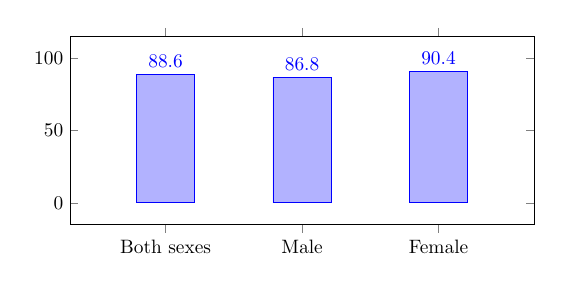
\begin{tikzpicture}[scale=0.7,transform shape]
\begin{axis}[
ybar,
width=10cm, 
height=5cm, 
enlarge y limits=0.15, enlarge x limits=0.35,
symbolic x coords={Both sexes, Male, Female},
xtick=data,
nodes near coords, nodes near coords align={vertical},
ymin=0,
ymax=100,
bar width=30pt,
]
\addplot coordinates {(Both sexes, 88.6) (Male, 86.8) (Female, 90.4)};
\end{axis}
\end{tikzpicture}
\captionof{figure}{Basic literacy rate of population 10 to 64 years by sex, Philippines 2003. Source: \url{http://62.0.5.133/www.census.gov.ph/data/sectordata/fl03_lsff2.gif}}\label{chap10fig:3}
\end{center}
\begin{center}
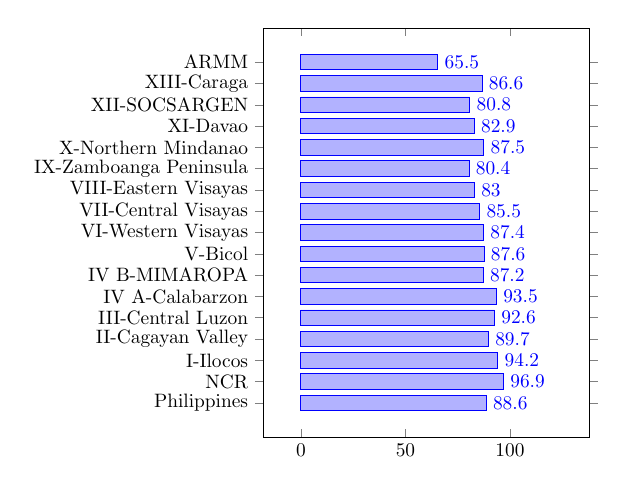
\begin{tikzpicture}[scale=0.7,transform shape]
\begin{axis}[
xbar,
width=7.5cm, 
height=9cm, 
enlarge x limits=0.15,
symbolic y coords={
Philippines,
NCR,
I-Ilocos,
II-Cagayan Valley,
III-Central Luzon,
IV A-Calabarzon,
IV B-MIMAROPA,
V-Bicol,
VI-Western Visayas,
VII-Central Visayas,
VIII-Eastern Visayas,
IX-Zamboanga Peninsula,
X-Northern Mindanao,
XI-Davao,
XII-SOCSARGEN,
XIII-Caraga,
ARMM
},
ytick=data,
nodes near coords, nodes near coords align={horizontal},
xmin=0,
xmax=120,
bar width=8pt,
]
\addplot coordinates {
(88.6,Philippines)
(96.9,NCR)
(94.2,I-Ilocos)
(89.7,II-Cagayan Valley)
(92.6,III-Central Luzon)
(93.5,IV A-Calabarzon)
(87.2,IV B-MIMAROPA)
(87.6,V-Bicol)
(87.4,VI-Western Visayas)
(85.5,VII-Central Visayas)
(83.0,VIII-Eastern Visayas)
(80.4,IX-Zamboanga Peninsula)
(87.5,X-Northern Mindanao)
(82.9,XI-Davao)
(80.8,XII-SOCSARGEN)
(86.6,XIII-Caraga)
(65.5,ARMM)
};
\end{axis}
\end{tikzpicture}
\captionof{figure}{Basic literacy rate of population 10 to 64 years by region, Philippines 2003. Source: \url{http://62.0.5.133/www.census.gov.ph/data/sectordata/fl03_lsff2.gif}}\label{chap10fig:4}
\end{center}

\item Below is a pie chart which shows the percentage of OFWs by place of work from April to
September 2000.

\begin{center}
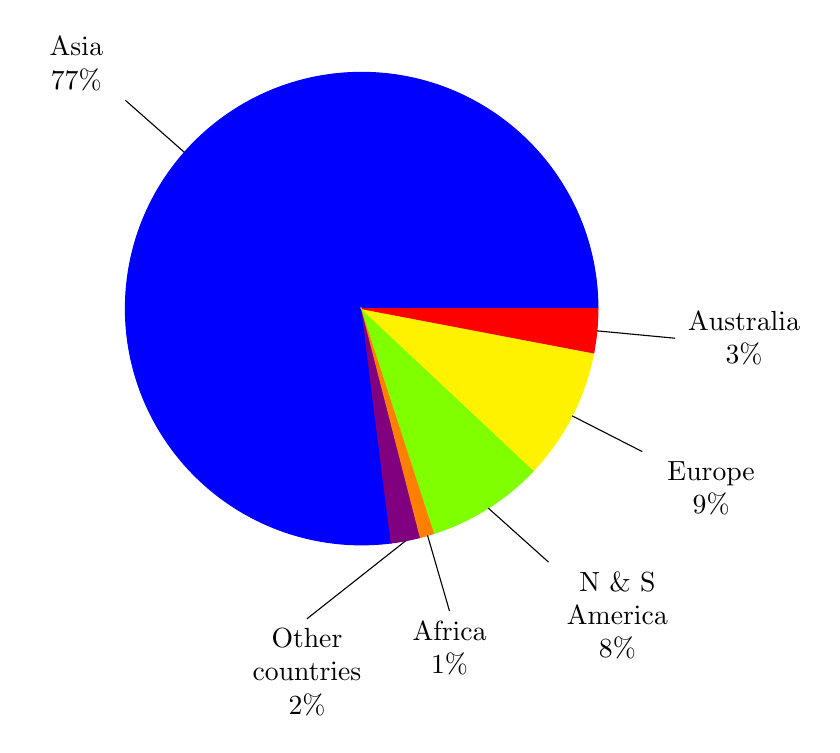
\begin{tikzpicture}[draw=black]
\tikzset{every fill/.style={opacity=0.5}}
\filldraw [blue] (0,0) -- (0:3cm) arc (0:277.2:3cm) -- cycle;
\filldraw [violet] (0,0) -- (277.2:3cm) arc (277.2:284.4:3cm) -- cycle;
\filldraw [orange] (0,0) -- (284.4:3cm) arc (284.4:288:3cm) -- cycle;
\filldraw [green!50!yellow] (0,0) -- (288:3cm) arc (288:316.8:3cm) -- cycle;
\filldraw [yellow] (0,0) -- (316.8:3cm) arc (316.8:349.2:3cm) -- cycle;
\filldraw [red] (0,0) -- (349.2:3cm) arc (349.2:360:3cm) -- cycle;
\draw (138.6:3cm) -- (138.6:4cm) node [above left,text width=1cm,align=center] {Asia 77\%};
\draw (280.8:3cm) -- (260:4cm) node [below,text width=1.5cm,align=center] {Other countries 2\%};
\draw (286.2:3cm) -- (286.2:4cm) node [below,text width=1.5cm,align=center] {Africa 1\%};
\draw (302.4:3cm) -- (306.4:4cm) node [below right,text width=1.5cm,align=center] {N \&{} S America 8\%};
\draw (333:3cm) -- (333:4cm) node [below right,text width=1.5cm,align=center] {Europe 9\%};
\draw (354.6:3cm) -- (354.6:4cm) node [right,text width=1.5cm,align=center] {Australia 3\%};
\end{tikzpicture}
\captionof{figure}{Percentage of OFWs by Place of Work: April to September 2000. Source: \url{http://www.census.gov.ph/}}\label{chap10fig:5}
\end{center}

What conclusion can you draw from the chart?

\item The data represent the monthly salary for a sample of government employees from
San Ildefonso, Ilocos Sur. Find the mean, median and mode.

\begin{center}
\begin{tabular}{lllll}
\textpeso 31,200 & \textpeso 23,500 & \textpeso 25,300 & \textpeso 31,200&  \textpeso 9,000\\
\textpeso 31,200 & \textpeso 8,000 & \textpeso 15,700 & \textpeso 16,300 & \textpeso 10,000\\
\textpeso 21,000 & \textpeso 9,500 & \textpeso 12,000 & \textpeso 16,000 & \textpeso 14,000\\
\end{tabular}
\end{center}

\item The ages of 40 teachers in a certain school are as follows:

\begin{center}
\begin{tabular}{cccccccccc}
43 & 58 & 21 & 24 & 31 & 49 & 40 & 51 & 55 & 28\\
50 & 33 & 62 & 30 & 25 & 39 & 59 & 29 & 36 & 42\\
38 & 46 & 42 & 52 & 26 & 50 & 41 & 37 & 35 & 40\\
47 & 35 & 57 & 55 & 36 & 45 & 32 & 45 & 42 & 36\\
\end{tabular}
\end{center}
   \begin{myenumerate}
	\item\label{chap10item:1} Set up a frequency distribution using 6 classes with the smallest starting at 21.
	\item Derive a cumulative frequency distribution for \eqref{chap10item:1}.
	\item Draw a histogram \eqref{chap10item:1}.
	\item Calculate the mean, median, and the mode of the distribution.
	\end{myenumerate}
\end{myenumerate}
\subsubsection*{MISLEADING STATISTICS}
Work with a group to explore how statistics can be misleading. Think about how the
data could be represented in other non-misleading way.
\begin{myenumerate}
\item Boy 1: Have you seen the poster outside this building saying

\begin{center}
\fbox{
\parbox[t][]{0.4\linewidth}{\centering
Electronic Load\\
Earn Money The Easiest Way\\
Average Php 2,000 per week\\
For information, call 888-02-02
}}
\end{center}

I think it will be suited for us.

Boy 2: Yes, but I doubt because it could be misleading.

\begin{enumerate}
\item Discuss reasons why the poster Boy 1 and Boy 2 saw could be misleading.
\item Create a hypothetical frequency table that indicates why the “average” earning of
Php 2,000 per week is a misleading statistic.
\end{enumerate}

\item A school head evaluates his colleagues in terms of some criteria. He gives O or
outstanding rating if his colleague averages 96-100, VS or very satisfactory if 90-95, S or
satisfactory if 85-89, and P or poor if 80-84. Teacher X got these scores: 90, 95, 80, 84,
98, and 83. The school head gave him an S. How might Teacher X convince the head
that he deserve a higher grade?

\item The bars on this graph appear to indicate that Salesgirl X has sold 3 times as many
garments as Salesgirl W. Salesgirl W appears to have sold twice as many as Salesgirl Y.
And the difference between the sales of Salesgirl X and Salesgirl Z is not very large.
\begin{enumerate}
\item Discuss why the graph is misleading.
\item Create a graph that accurately reflects the data.
\begin{center}
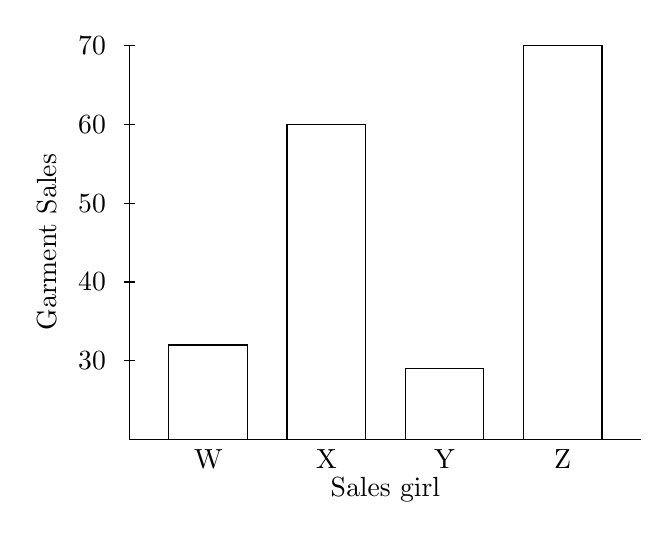
\begin{tikzpicture}
\draw (0,0) -- (0,5);
\draw (0,0) -- (6.5,0);
\foreach \y/\ytext in {1/30,2/40,3/50,4/60,5/70}
	\node [left=5pt] at (0,\y) {\ytext};
\foreach \y in {1,2,3,4,5}
	\draw (-2pt,\y) -- (2pt,\y);
\draw (0.5,0) rectangle (1.5, 1.2);
\draw (2,0) rectangle (3, 4);
\draw (3.5,0) rectangle (4.5,.9);
\draw (5,0) rectangle (6,5);
\foreach \x/\xtext in {1/W,2.5/X,4/Y,5.5/Z}
	\node [below] at (\x,0) {\xtext};
\node [below=10pt] at (3.25,0) {Sales girl};
\node [left=30pt,yshift=1.25cm,rotate=90] at (0,2.5) {Garment Sales};
\end{tikzpicture}
\end{center}
\end{enumerate}
\end{myenumerate}

\subsubsection*{CARRYING OUT A SURVEY}
This is to formalize the learnings you gained from this module. The objectives of
the activity are the following:
\begin{enumerate}
\item To conduct a simple survey from your co-participants.
\item To prepare a graphical or tabular presentation of your survey.
\end{enumerate}

\paragraph*{Procedure}
\begin{enumerate}
\item Group yourselves into 5. Work together to write a plan for a survey using questionnaire
method.
\item Think of any topic that is of interest to you and construct a questionnaire.
\item The plan should include: title of the survey, purpose, importance of what you want to
do, population and sample, and the questionnaire.
\item Conduct the survey.
\item Prepare the graphical or tabular presentation of your survey.
\item Make inference and necessary conclusions on your survey.
\end{enumerate}
